% Options for packages loaded elsewhere
\PassOptionsToPackage{unicode}{hyperref}
\PassOptionsToPackage{hyphens}{url}
\PassOptionsToPackage{dvipsnames,svgnames,x11names}{xcolor}
%
\documentclass[
true
]{sn-jnl}

\usepackage{amsmath,amssymb}
\usepackage{iftex}
\ifPDFTeX
  \usepackage[T1]{fontenc}
  \usepackage[utf8]{inputenc}
  \usepackage{textcomp} % provide euro and other symbols
\else % if luatex or xetex
  \usepackage{unicode-math}
  \defaultfontfeatures{Scale=MatchLowercase}
  \defaultfontfeatures[\rmfamily]{Ligatures=TeX,Scale=1}
\fi
\usepackage{lmodern}
\ifPDFTeX\else  
    % xetex/luatex font selection
\fi
% Use upquote if available, for straight quotes in verbatim environments
\IfFileExists{upquote.sty}{\usepackage{upquote}}{}
\IfFileExists{microtype.sty}{% use microtype if available
  \usepackage[]{microtype}
  \UseMicrotypeSet[protrusion]{basicmath} % disable protrusion for tt fonts
}{}
\makeatletter
\@ifundefined{KOMAClassName}{% if non-KOMA class
  \IfFileExists{parskip.sty}{%
    \usepackage{parskip}
  }{% else
    \setlength{\parindent}{0pt}
    \setlength{\parskip}{6pt plus 2pt minus 1pt}}
}{% if KOMA class
  \KOMAoptions{parskip=half}}
\makeatother
\usepackage{xcolor}
\setlength{\emergencystretch}{3em} % prevent overfull lines
\setcounter{secnumdepth}{5}
% Make \paragraph and \subparagraph free-standing
\makeatletter
\ifx\paragraph\undefined\else
  \let\oldparagraph\paragraph
  \renewcommand{\paragraph}{
    \@ifstar
      \xxxParagraphStar
      \xxxParagraphNoStar
  }
  \newcommand{\xxxParagraphStar}[1]{\oldparagraph*{#1}\mbox{}}
  \newcommand{\xxxParagraphNoStar}[1]{\oldparagraph{#1}\mbox{}}
\fi
\ifx\subparagraph\undefined\else
  \let\oldsubparagraph\subparagraph
  \renewcommand{\subparagraph}{
    \@ifstar
      \xxxSubParagraphStar
      \xxxSubParagraphNoStar
  }
  \newcommand{\xxxSubParagraphStar}[1]{\oldsubparagraph*{#1}\mbox{}}
  \newcommand{\xxxSubParagraphNoStar}[1]{\oldsubparagraph{#1}\mbox{}}
\fi
\makeatother


\providecommand{\tightlist}{%
  \setlength{\itemsep}{0pt}\setlength{\parskip}{0pt}}\usepackage{longtable,booktabs,array}
\usepackage{calc} % for calculating minipage widths
% Correct order of tables after \paragraph or \subparagraph
\usepackage{etoolbox}
\makeatletter
\patchcmd\longtable{\par}{\if@noskipsec\mbox{}\fi\par}{}{}
\makeatother
% Allow footnotes in longtable head/foot
\IfFileExists{footnotehyper.sty}{\usepackage{footnotehyper}}{\usepackage{footnote}}
\makesavenoteenv{longtable}
\usepackage{graphicx}
\makeatletter
\newsavebox\pandoc@box
\newcommand*\pandocbounded[1]{% scales image to fit in text height/width
  \sbox\pandoc@box{#1}%
  \Gscale@div\@tempa{\textheight}{\dimexpr\ht\pandoc@box+\dp\pandoc@box\relax}%
  \Gscale@div\@tempb{\linewidth}{\wd\pandoc@box}%
  \ifdim\@tempb\p@<\@tempa\p@\let\@tempa\@tempb\fi% select the smaller of both
  \ifdim\@tempa\p@<\p@\scalebox{\@tempa}{\usebox\pandoc@box}%
  \else\usebox{\pandoc@box}%
  \fi%
}
% Set default figure placement to htbp
\def\fps@figure{htbp}
\makeatother

%%%% Standard Packages

\usepackage{graphicx}%
\usepackage{multirow}%
\usepackage{amsmath,amssymb,amsfonts}%
\usepackage{amsthm}%
\usepackage{mathrsfs}%
\usepackage[title]{appendix}%
\usepackage{xcolor}%
\usepackage{textcomp}%
\usepackage{manyfoot}%
\usepackage{booktabs}%
\usepackage{algorithm}%
\usepackage{algorithmicx}%
\usepackage{algpseudocode}%
\usepackage{listings}%

%%%%

\raggedbottom
\makeatletter
\@ifpackageloaded{caption}{}{\usepackage{caption}}
\AtBeginDocument{%
\ifdefined\contentsname
  \renewcommand*\contentsname{Table of contents}
\else
  \newcommand\contentsname{Table of contents}
\fi
\ifdefined\listfigurename
  \renewcommand*\listfigurename{List of Figures}
\else
  \newcommand\listfigurename{List of Figures}
\fi
\ifdefined\listtablename
  \renewcommand*\listtablename{List of Tables}
\else
  \newcommand\listtablename{List of Tables}
\fi
\ifdefined\figurename
  \renewcommand*\figurename{\textbf{Figure}}
\else
  \newcommand\figurename{\textbf{Figure}}
\fi
\ifdefined\tablename
  \renewcommand*\tablename{\textbf{Table}}
\else
  \newcommand\tablename{\textbf{Table}}
\fi
}
\@ifpackageloaded{float}{}{\usepackage{float}}
\floatstyle{ruled}
\@ifundefined{c@chapter}{\newfloat{codelisting}{h}{lop}}{\newfloat{codelisting}{h}{lop}[chapter]}
\floatname{codelisting}{Listing}
\newcommand*\listoflistings{\listof{codelisting}{List of Listings}}
\captionsetup{labelsep=period}
\makeatother
\makeatletter
\makeatother
\makeatletter
\@ifpackageloaded{caption}{}{\usepackage{caption}}
\@ifpackageloaded{subcaption}{}{\usepackage{subcaption}}
\makeatother

\usepackage[]{natbib}
\bibliographystyle{plainnat}
\usepackage{bookmark}

\IfFileExists{xurl.sty}{\usepackage{xurl}}{} % add URL line breaks if available
\urlstyle{same} % disable monospaced font for URLs
\hypersetup{
  pdftitle={Does the Brain's E/I Balance Really Shape Long-Range Temporal Correlations?},
  pdfauthor={, and },
  pdfkeywords={Hurst exponent, long range temporal
correlation, excitatory / inhibitory balance, criticality, complex
systems, visual task, functional magnetic resnonance imaging, magnetic
resonance spectroscopy},
  colorlinks=true,
  linkcolor={blue},
  filecolor={Maroon},
  citecolor={Blue},
  urlcolor={Blue},
  pdfcreator={LaTeX via pandoc}}


\title[Does the Brain's E/I Balance Really Shape Long-Range Temporal
Correlations?]{Does the Brain's E/I Balance Really Shape Long-Range
Temporal Correlations?}

% author setup
\author[1]{\fnm{Lydia} \sur{Sochan}}\email{lydiasochan@gmail.com}\author*[1,2,3]{\fnm{Alexander Mark} \sur{Weber}}\email{aweber@bcchr.ca}
% affil setup
\affil[1]{, \orgname{School of Biomedical Engineering, The University of
British Columbia, Vancouver, BC, Canada}}
\affil[2]{, \orgname{BC Children's Hospital Research Institute, The
University of British Columbia, Vancouver, BC, Canada}}
\affil[3]{, \orgname{Pediatrics, The University of British Columbia,
Vancouver, BC, Canada}}

% abstract 


% keywords
\keywords{Hurst exponent,  long range temporal correlation,  excitatory
/ inhibitory balance,  criticality,  complex systems,  visual
task,  functional magnetic resnonance imaging,  magnetic resonance
spectroscopy}

\begin{document}
\maketitle


\textsuperscript{1} School of Biomedical Engineering, The University of
British Columbia, Vancouver, BC, Canada\\
\textsuperscript{2} BC Children's Hospital Research Institute, The
University of British Columbia, Vancouver, BC, Canada\\
\textsuperscript{3} Pediatrics, The University of British Columbia,
Vancouver, BC, Canada

\textsuperscript{*} Correspondence:
\href{mailto:aweber@bcchr.ca}{Alexander Mark Weber
\textless{}aweber@bcchr.ca\textgreater{}}

\subsection*{Abstract}\label{abstract}
\addcontentsline{toc}{subsection}{Abstract}

\section{Introduction}\label{introduction}

Thirty years ago, functional magnetic resonance imaging (fMRI)
profoundly changed the world of MRI by allowing real-time analysis of
pressing neuropsychological questions
\citep{ogawaMagneticResonanceImaging1990, ogawaBrainMagneticResonance1990, stephanShortHistoryCausal2012}.
While initially used to probe task-based responses, researchers have
more recently developed an interest in studying brain function at rest,
known as resting-state fMRI (rs-fMRI)
\citep{decoRestingBrainsNever2013}, i.e.~to understand how brain
dynamics at rest are related to neurological functioning as well as
individual differences. A critical tool in analyzing these dynamics is
the Hurst exponent (H)
\citep{campbellMonofractalAnalysisFunctional2022}, a measure of
self-similarity derived from the blood-oxygen-dependent (BOLD) signal. H
estimates the extent to which the BOLD signal displays long-term memory,
where a higher value indicates a self-similar signal with long-term
positive autocorrelations
\citep{campbellMonofractalAnalysisFunctional2022, beggsBeingCriticalCriticality2012}.
Another way of understanding H is that a signal with high H is fractal:
similar temporal signal fluctuations are observed, no matter the time
scale \citep{campbellMonofractalAnalysisFunctional2022}.

H has also emerged as a valuable tool in clinical research, capturing
changes in BOLD signal dynamics across various neuropsychiatric
conditions. In aging populations for instance, H has been found to be
elevated
\citep{dongHurstExponentAnalysis2018, winkAgeCholinergicEffects2006};
this relationship has also been found in mild cognitive impairment and
Alzheimer's disease
\citep{maximFractionalGaussianNoise2005, longBrainnetomeAtlasBased2018}.
Additionally, changes in H have been observed in conditions such as
autism, mood disorders, and brain injury
\citep{laiShiftRandomnessBrain2010, donaTemporalFractalAnalysis2017, weiIdentifyingMajorDepressive2013, jingIdentifyingCurrentRemitted2017, donaFractalAnalysisBrain2017}.
These differences suggest H may reflect changes in global and local
functioning.

Underlying these observations is the critical brain hypothesis, which
posits that the brain operates at a critical point, a state where order
and disorder are perfectly balanced to enable optimal information
processing
\citep{decoRestingBrainsNever2013, beggsBeingCriticalCriticality2012, barangerChaosComplexityEntropy2000, bassettUnderstandingComplexityHuman2011, zimmernWhyBrainCriticality2020, liangExcitationInhibitionBalance2024, poilCriticalStateDynamicsAvalanches2012, lombardiBalanceExcitationInhibition2017, baumgartenCriticalExcitationinhibitionBalance2019, bruiningMeasurementExcitationinhibitionRatio2020, trakoshisIntrinsicExcitationinhibitionImbalance, gaoInferringSynapticExcitation2017, tianTheoreticalFoundationsStudying2022, rubinovNeurobiologicallyRealisticDeterminants2011}.
When operating at a critical point, the brain is maximally sensitive to
external stimuli, and can dynamically transition between ordered and
disordered states to promote efficient cognitive processing
\citep{decoRestingBrainsNever2013, beggsBeingCriticalCriticality2012, tianTheoreticalFoundationsStudying2022, rubinovNeurobiologicallyRealisticDeterminants2011}.Recent
papers suggest the control parameter underlying the brain's ability to
transition between states is the excitatory-inhibitory (E/I) ratio, the
balance of excitatory and inhibitory neural activity, often
operationalized as the ratio of the primary excitatory-to-inhibitory
neurotransmitters, i.e.~glutamate-to-GABA ratio
\citep{liangExcitationInhibitionBalance2024, lombardiBalanceExcitationInhibition2017, baumgartenCriticalExcitationinhibitionBalance2019, bruiningMeasurementExcitationinhibitionRatio2020, trakoshisIntrinsicExcitationinhibitionImbalance, gaoInferringSynapticExcitation2017}.
It is thought that E/I controls criticality by modulating the brain's
signal-to-noise ratio
\citep{liangExcitationInhibitionBalance2024, rubensteinModelAutismIncreased2003}.

Besides the implications to the critical brain hypothesis, understanding
if E/I is related to H may allow for easier estimation of excitatory and
inhibitory neurotransmitters, as accurate E/I measurement is technically
challenging \citep{ajramContribution1HMagnetic2019}. Magnetic resonance
spectroscopy (MRS) is the only non-invasive method of measuring the
ratio of glutamate (Glu; excitatory) to Gamma-aminobutyric acid (GABA;
inhibitory) \emph{in vivo}
\citep{stanleyFunctionalMagneticResonance2018}. Unfortunately, it has
both limited spatial and temporal resolution
\citep{gaoInferringSynapticExcitation2017, ajramContribution1HMagnetic2019, stanleyFunctionalMagneticResonance2018}.
Consequently, if H could serve as a proxy for E/I, it would be much
easier to estimate E/I in conditions of interest such as autism,
Alzheimer's, and schizophrenia.

There are a handful of studies suggesting a link between H and E/I,
however they are all either computational models or animal studies
\citep{liangExcitationInhibitionBalance2024, poilCriticalStateDynamicsAvalanches2012, lombardiBalanceExcitationInhibition2017, baumgartenCriticalExcitationinhibitionBalance2019, bruiningMeasurementExcitationinhibitionRatio2020, trakoshisIntrinsicExcitationinhibitionImbalance, gaoInferringSynapticExcitation2017}.
Moreover, their findings are inconsistent, with some reporting positive
linear, negative linear, or U-shaped relationships between the two
variables (see Table~\ref{tbl-lit}). Thus, there is a need for further
study, both to clarify the nature of a potential E/I-Hurst relationship,
and also to confirm if this relationship indeed exists in the human
brain. Therefore, the current study seeks to investigate the potential
E/I-Hurst relationship in vivo, within the visual cortex during
movie-watching and rest.

\begin{longtable}[]{@{}
  >{\raggedright\arraybackslash}p{(\linewidth - 10\tabcolsep) * \real{0.1585}}
  >{\raggedright\arraybackslash}p{(\linewidth - 10\tabcolsep) * \real{0.1707}}
  >{\raggedright\arraybackslash}p{(\linewidth - 10\tabcolsep) * \real{0.1707}}
  >{\raggedright\arraybackslash}p{(\linewidth - 10\tabcolsep) * \real{0.1585}}
  >{\raggedright\arraybackslash}p{(\linewidth - 10\tabcolsep) * \real{0.1707}}
  >{\raggedright\arraybackslash}p{(\linewidth - 10\tabcolsep) * \real{0.1707}}@{}}
\caption{Summary of methods for existing E/I-Hurst
studies}\label{tbl-lit}\tabularnewline
\toprule\noalign{}
\begin{minipage}[b]{\linewidth}\raggedright
Citation
\end{minipage} & \begin{minipage}[b]{\linewidth}\raggedright
Study Type
\end{minipage} & \begin{minipage}[b]{\linewidth}\raggedright
H Data Type
\end{minipage} & \begin{minipage}[b]{\linewidth}\raggedright
H Calculation Method
\end{minipage} & \begin{minipage}[b]{\linewidth}\raggedright
E/I Type
\end{minipage} & \begin{minipage}[b]{\linewidth}\raggedright
E/I-Hurst Relationship
\end{minipage} \\
\midrule\noalign{}
\endfirsthead
\toprule\noalign{}
\begin{minipage}[b]{\linewidth}\raggedright
Citation
\end{minipage} & \begin{minipage}[b]{\linewidth}\raggedright
Study Type
\end{minipage} & \begin{minipage}[b]{\linewidth}\raggedright
H Data Type
\end{minipage} & \begin{minipage}[b]{\linewidth}\raggedright
H Calculation Method
\end{minipage} & \begin{minipage}[b]{\linewidth}\raggedright
E/I Type
\end{minipage} & \begin{minipage}[b]{\linewidth}\raggedright
E/I-Hurst Relationship
\end{minipage} \\
\midrule\noalign{}
\endhead
\bottomrule\noalign{}
\endlastfoot
Poil et al.~(2012)\citet{poilCriticalStateDynamicsAvalanches2012} &
Computational with in-house simulated model & Neuronal avalanche size &
Detrendend fluctuation analysis (DFA) & Structural: number of E-to-I
neurons & Inverse U \\
Bruining et
al.~(2020)\citet{bruiningMeasurementExcitationinhibitionRatio2020} &
Computational with model by Poil et al.~(2012); modified in-house &
Neuronal oscillation amplitude & DFA & Structural: number of E-to-I
synapses & Inverse U \\
Gao et al.~(2017)\citet{gaoInferringSynapticExcitation2017} &
Computational; in vivo in rats and macaques & Local field potential
(LFP) & PSD & Estimated from LFP & Positive linear \\
Lombardi et al.~(2017)\citet{lombardiBalanceExcitationInhibition2017} &
Computational with in-house model & Neuronal avalanche size & PSD &
Structural: number of E-to-I neurons & Negative linear \\
Trakoshis et
al.~(2020)\citet{trakoshisIntrinsicExcitationinhibitionImbalance} &
Computational with simulated data; in vivo in mice & fMRI BOLD signal &
Wavelet-based maximum likelihood method & E-to-I synaptic conductance &
Positive linear \\
\end{longtable}

\section{Methods}\label{methods}

\subsection{Participants}\label{participants}

Twenty-seven healthy adult participants were recruited to the study. One
participant was not scanned due to feelings of claustrophobia while in
the scanner. After our analysis and performing quality assurance (see
below), a further seven participants were removed for having less than
ideal MRI data quality, leaving nineteen final participants, between the
ages of 21.3 and 53.4 (mean age ± sd: 30.1 ± 8.7 years; 9 males).

\subsection{Ethics Statement}\label{ethics-statement}

Written informed consent was obtained from all participants. Ethics
approval was granted by the Clinical Research Ethics Board at the
University of British Columbia and BC Children's \& Women's Hospital
(H21-02686).

\subsection{Scanning Procedure}\label{scanning-procedure}

After two anatomical sequences were acquired, participants were
instructed to visually fixate on a cross-hair for 24 minutes. During
this period, an fMRI, MEGA-PRESS, and sLASER sequence were acquired (see
Figure~\ref{fig-method} A and Section~\ref{sec-mriacq}). Next,
participants were instructed to watch a nature documetnary (Our Planet
(2019), Episode 3, ``Jungles'' \citet{cordeyJungles2019}) for 24
minutes. During this period, another set of fMRI, sLASER, and MEGA-PRESS
sequences were acquired. See Figure~\ref{fig-method} B for a visual
representation of the scanning protocol. Total scan duration was
approximately 1 hour. All participants followed the same order of rest
than movie, and all participants saw the same movie segment, beginning
at the same time during the scan.

\phantomsection\label{cell-fig-method}
\begin{figure}[H]

\centering{

\pandocbounded{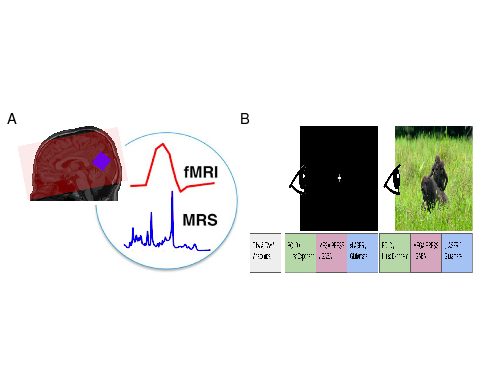
\includegraphics[keepaspectratio]{index_files/figure-pdf/fig-method-1.pdf}}

}

\caption{\label{fig-method}\textbf{Overview of the MRI acquisition
protocol.} A) fMRI coverage was across the whole-brain (example coverage
in red). MRS voxels were placed in the visual cortex (blue). Background
image is of a T1w acquisition from a sample subject. B) fMRI, MEGA-PRESS
and sLASER were acquired first with participants looking at a white
cross for 24 mintues. Next, the same sequences were acquired with the
participants viewing a nature documentary for an identical period of
time.}

\end{figure}%

\subsection{Acquisition Details}\label{sec-mriacq}

Scans were performed at BC Children's Hospital MRI Research Facility on
a 3.0 Tesla GE Discovery MR750 scanner (scanner software version:
DV26.0\_R03) with a Nova Medical 32 channel head coil. Participants
changed into scrubs and were screened by an MRI technologist.
Participants were given wax earplugs and a fiducial was placed on their
left temple. Participants were provided with an audio headset and
blanket once lying down on the scanner bed. Since visual stimuli were to
be rear-projected, position and angle of mirror above patient eyes was
adjusted for optimal movie viewing.

The following MRI scans were acquired. A 3D T1-weighted sagittal fast
spoiled gradient echo (FSPGR) sequence; a 3D T2-weighted sagittal CUBE;
a 2D echo-planar imaging (EPI) multi-echo gradient-echo fMRI sequence; a
semi-LASER (sLASER) sequence; and a MEGA-PRESS sequence. Details are
listed in Table~\ref{tbl-mriacq}.

\begin{longtable}[]{@{}
  >{\raggedright\arraybackslash}p{(\linewidth - 14\tabcolsep) * \real{0.1886}}
  >{\raggedright\arraybackslash}p{(\linewidth - 14\tabcolsep) * \real{0.0857}}
  >{\raggedright\arraybackslash}p{(\linewidth - 14\tabcolsep) * \real{0.0686}}
  >{\raggedright\arraybackslash}p{(\linewidth - 14\tabcolsep) * \real{0.0686}}
  >{\raggedright\arraybackslash}p{(\linewidth - 14\tabcolsep) * \real{0.0914}}
  >{\raggedright\arraybackslash}p{(\linewidth - 14\tabcolsep) * \real{0.1257}}
  >{\raggedright\arraybackslash}p{(\linewidth - 14\tabcolsep) * \real{0.1600}}
  >{\raggedright\arraybackslash}p{(\linewidth - 14\tabcolsep) * \real{0.2114}}@{}}
\caption{Summary of MRI acquisition
details}\label{tbl-mriacq}\tabularnewline
\toprule\noalign{}
\begin{minipage}[b]{\linewidth}\raggedright
Sequence
\end{minipage} & \begin{minipage}[b]{\linewidth}\raggedright
TE (ms)
\end{minipage} & \begin{minipage}[b]{\linewidth}\raggedright
TR (ms)
\end{minipage} & \begin{minipage}[b]{\linewidth}\raggedright
Flip Angle
\end{minipage} & \begin{minipage}[b]{\linewidth}\raggedright
FOV
\end{minipage} & \begin{minipage}[b]{\linewidth}\raggedright
Slice Thickness (mm)
\end{minipage} & \begin{minipage}[b]{\linewidth}\raggedright
In-Plane Resolution (mm²)
\end{minipage} & \begin{minipage}[b]{\linewidth}\raggedright
Other Parameters
\end{minipage} \\
\midrule\noalign{}
\endfirsthead
\toprule\noalign{}
\begin{minipage}[b]{\linewidth}\raggedright
Sequence
\end{minipage} & \begin{minipage}[b]{\linewidth}\raggedright
TE (ms)
\end{minipage} & \begin{minipage}[b]{\linewidth}\raggedright
TR (ms)
\end{minipage} & \begin{minipage}[b]{\linewidth}\raggedright
Flip Angle
\end{minipage} & \begin{minipage}[b]{\linewidth}\raggedright
FOV
\end{minipage} & \begin{minipage}[b]{\linewidth}\raggedright
Slice Thickness (mm)
\end{minipage} & \begin{minipage}[b]{\linewidth}\raggedright
In-Plane Resolution (mm²)
\end{minipage} & \begin{minipage}[b]{\linewidth}\raggedright
Other Parameters
\end{minipage} \\
\midrule\noalign{}
\endhead
\bottomrule\noalign{}
\endlastfoot
\textbf{3D T1-weighted FSPGR} & 2.176 & 7.216 & 12 & 256 × 256 & 0.9 &
0.9375 × 0.9375 & - \\
\textbf{3D T2-weighted CUBE} & 75.242 & 2,504.0 & 90 & 256 x 256 & 0.9 &
0.9375 × 0.9375 & - \\
\textbf{2D EPI Multi-Echo fMRI} & 12.2, 35.352, 58.504 & 1,500 & 52 & 64
x 64 & 3.6 & 3.5938 × 3.5938 & Acceleration factor = 6 \\
\textbf{sLASER} & 35 & 2,000 & 90 & - & 28.0 & 28.0 x 28.0 & - \\
\textbf{MEGA-PRESS} & 68 & 1,800 & 90 & - & 28.0 & 28.0 x 28.0 & - \\
\end{longtable}

For both MRS sequences, the voxel size was set to 2.8 x 2.8 x 2.8
cm\textsuperscript{3}. MRS voxels were rotated and placed in the
occipital lobe, aligned along the calcarine fissure. Finally, blip-up
and blip-down spin-echo versions of the fMRI sequence were acquired at
the end to estimate the B0 non-uniformity map for fMRI phase distortion
correction.

\subsection{Image Processing}\label{image-processing}

Our full image processing pipeline has been can be accessed from our
Github account page:
\href{https://github.com/WeberLab/EI_Hurst_Analysis}{github.com/WeberLab/EI\_Hurst\_Analysis}

Images were downloaded offline from the scanner in raw Digital Imaging
and Communications in Medicine (DICOM) format. DICOM files were then
converted to Neuroimaging Informatics Technology Initiative (NIfTI)
using Chris Rorden's \texttt{dcm2niix}
\citep{liFirstStepNeuroimaging2016} (v1.0.20211006) and then to Brain
Imaging Data Structure (BIDS) \citep{gorgolewskiBrainImagingData2016}
format using \texttt{dcm2bids} \citep{boreDcm2Bids2023} (v2.1.6).

\subsubsection{Structural Images}\label{structural-images}

The T1w image was corrected for intensity non-uniformity with
\texttt{N4BiasFieldCorrection} \citep{tustisonN4ITKImprovedN32010} and
distributed using \texttt{ANTs}
\citep{avantsSymmetricDiffeomorphicImage2008} (v2.3.335) to be used as a
T1w-reference for the rest of the workflow. The T1w-reference was
skull-stripped using a \texttt{Nipype}
\citep{gorgolewskiNipypeFlexibleLightweight2016} implementation of
\texttt{antsBrainExtraction.sh} from \texttt{ANTs}; \texttt{OASIS30ANTs}
was used as a target template. \texttt{Fast}
\citep{zhangSegmentationBrainMR2001} (\texttt{FSL}
\citep{smithAdvancesFunctionalStructural2004} v.6.0.5.1:57b01774, RRID:
SCR\_002823) was used for brain tissue segmentation into cerebrospinal
fluid (CSF), white matter (WM), and gray matter (GM). Brain surfaces
were reconstructed with \texttt{recon-all}
\citep{daleCorticalSurfacebasedAnalysis1999} (\texttt{FreeSurfer}
\citep{daleCorticalSurfacebasedAnalysis1999} 7.3.2, RRID: SCR\_001847).
The previously-estimated brain mask was refined with \texttt{Mindboggle}
\citep{kleinMindbogglingMorphometryHuman2017} (RRID:SCR\_002438) to
reconcile ANTs-derived and FreeSurfer-derived segmentations of cortical
GM. \texttt{AntsRegistration}
\citep{avantsSymmetricDiffeomorphicImage2008} (\texttt{ANTs} 2.3.3) was
used to perform volume-based spatial normalization to two standard
spaces: MNI152NLin2009cAsym and MNI152NLin6Asym. Normalization used
brain-extracted versions of both T1w reference and T1w template.

\subsubsection{fMRI}\label{fmri}

Using \texttt{fMRIPrep} \citep{estebanFMRIPrepRobustPreprocessing2019},
the shortest echo of the BOLD run was used to generate a reference
volume (both skull-stripped and skull-included). Head-motion parameters
with respect to the BOLD reference (transformation matrices as well as
six corresponding rotation and translation parameters) were estimated
before spatiotemporal filtering using \texttt{mcflirt}
\citep{jenkinsonImprovedOptimizationRobust2002} (\texttt{FSL}
v6.0.5.1:57b01774). The fieldmap was aligned with rigid registration to
the target EPI reference run. Field coefficients were mapped to the
reference EPI using the transform. BOLD runs were slice-time corrected
to 643 ms (half of slice acquisitio range of 0-1290 ms) using
\texttt{3dTshift} from \texttt{AFNI} \citep{coxAFNISoftwareAnalysis1996}
(RRIS: SCR\_005927). To estimate T2* map from preprocessed EPI echoes, a
voxel-wise fitting was performed by fitting the maximum number of echoes
with reliable echoes in a particular voxel to a monoexponential signal
decay model with nonlinear regression. Initial values were T2\emph{/S0
estimates from a log-linear regression fit. This calculated T2} map was
then used to optimally combine preprocessed BOLD across echoes using the
method by Posse et al.~(1999)
\citep{posseEnhancementBOLDcontrastSensitivity1999}. The generated BOLD
reference was then co-registered (6 degrees of freedom) to the T1w
reference with \texttt{bbregister} (\texttt{FreeSurfer}
\citep{daleCorticalSurfacebasedAnalysis1999}) using boundary-based
registration. First, a reference volume and its skull-stripped
equivalent were generated with \texttt{fMRIPrep}. Confounding time
series were calculated from preprocessed BOLD: framewise displacement
(FD), DVARS, and three region-wise global signals. \texttt{Tedana}
\citep{dupreTEdependentAnalysisMultiecho2021} was then used to denoise
the data by decomposing the multi-echo BOLD data via principal component
analysis (PCA) and independent component analysis (ICA). The resulting
components are automatically analyzed to determine whether they are
TE-dependent or -independent. TE-dependent components were classified as
BOLD, while TE-independent components were classified as non-BOLD and
were discarded as part of data cleaning.

Participants were excluded from further ananlysis if their mean FD was
\textgreater{} 0.15 mm.

\subsection{MRS}\label{mrs}

sLASER data were processed and fit to a spectrum using \texttt{Osprey}
\citep{oeltzschnerOspreyOpenSourceProcessing2020} (v2.4.0). Full width
half-maximum (FWHM) of the single-Lorentzian fit of the
N-acetylaspartate (NAA) peak were calculated for quality assurance
purposes. The MRS voxel was co-registered to T1w reference image and
segmented by SPM12 \citep{fristonStatisticalParametricMapping2007} into
CSF, GM, and WM. Metabolites were water-scaled as well as tissue- and
relaxation-corrected by the Gasparovic et al.~(2006) method
\citep{gasparovicUseTissueWater2006}. Processed (non-fitted) data from
\texttt{Osprey} was also fed to \texttt{LCModel}
\citep{provencherAutomaticQuantitationLocalized2001} (v6.1) for fitting.
Cramer-Rao lower bounds (CRLBs) were calculated from LCModel fit.
\texttt{Osprey} estimates were used for further analysis. Glutamate is
challenging to capture due to its signal overlaps with other metabolites
\citep{pasantaFunctionalMRSStudies2023}. In particular, Glu shares a
similar chemical structure with glutamine (Gln) which causes the
spectral features of Glu to be contaminated with Gln
\citep{ramadanGlutamateGlutamineReview2013}. As a result, we decided to
report Glx values, which co-reports Glu and Gln to avoid errors in
spectral assignment, especially since it is controversial whether Glu
can reliably be separated from Gln at 3T
\citep{pasantaFunctionalMRSStudies2023, ramadanGlutamateGlutamineReview2013}.
We henceforth refer to Glu as either Glx or glutamate.

MEGA-PRESS data were processed and fit with \texttt{Osprey} and
\texttt{LCModel} as previously described (see Figure 5). Data were also
fit with \texttt{Gannet} (v3.3.0); they were relaxation-, tissue- and
alpha-corrected using the Harris et al.~(2015) method
\citep{harrisSpectralEditingMeasurementsGABA2015}. \texttt{Osprey}
values were ultimately used for further analysis. Due to the J-editing
sequence of MEGA-PRESS, a challenge of GABA quantification is
macromolecule quantification
\citep{harrisSpectralEditingMeasurementsGABA2015}. As a result, we
report GABA+, a measure which co-reports GABA with macromolecules.
Macromolecules (MM) are expected to account for approximately 45\% of
the GABA+ signal \citep{harrisSpectralEditingMeasurementsGABA2015}.
While a macromolecule-suppressed estimate of GABA seems ideal, a recent
25-site and multi-vendor study conducted at 3T found that GABA+ showed
much lower coefficient of variation than MM-suppressed GABA, meaning
that GABA+ is more consistent across research sites and MRI vendors
(i.e., Philips, GE, Siemens) \citep{mikkelsenBigGABAII2019}. Moreover,
GABA+ showed greater reliability for both creatine-referenced and
water-suppressed estimates
\citep{mikkelsenBigGABAEdited2017, mikkelsenBigGABAII2019}. MM-supressed
GABA and GABA+ estimates are also correlated, albeit weakly- to
moderately-so
\citep{harrisSpectralEditingMeasurementsGABA2015, mikkelsenBigGABAII2019, mikkelsenBigGABAEdited2017}.
Consequently, we report GABA+ (henceforth referred to as GABA) to allow
for easier comparison of our results to other studies as well as
reproducibility.

Basis sets were created using \texttt{MRSCloud}
\citep{huiMRSCloudCloudbasedMRS2022, moriMRICloudDeliveringHighThroughput2016}.
For sLASER, `localization' was set to `sLASER', `vendor' to `GE',
`editing' to `UnEdited', and `TE' to 35. For MEGA-PRESS, `localization'
was set to `PRESS', `editing' to `MEGA', `TE' to 68, `edit on' to `1.9',
`edit off' to `7.5', and `pulse duration' to `14'. Metabolites included
for both basis sets were: Asc, Asp, Cr, CrCH2, EA, GABA, GPC, GSH, Gln,
Glu, Gly, H2O, Lac, NAA, NAAG, PCh, PCr, PE, Ser, Tau, mI, and sI.
Excitatory-inhibitory ratio (E/I) was calculated as {[}Glx in
i.u.{]}/{[}GABA+ in i.u.{]}, a common practice to report E/I using MRS
\citep{rideauxNoBalanceGlutamate+glutamine2021}.

Participants were excluded from further analysis if any of their MRS
scans had FWHM \textgreater{} 10. Originally we intended to calculate,
report and analyze MRS as tissue-corrected quantitative values. However,
the \texttt{Osprey} software was reporting Glx values that were an order
of magnitude larger than reported Glx values in the literature. Despite
several attempts, we were unable to locate the source of this error.
Therefore we decided to use Glx/Cr and GABA+/Cr values to be safe.

\subsection{Hurst Exponent
Calculation}\label{hurst-exponent-calculation}

Hurst exponent was calculated from the power spectrum density (PSD) of
the BOLD signal. A log-log plot was used, where log power was plotted
against log frequency; generally, if a log-log plot results in a linear
relationship, it is assumed that the mean slope of this line represents
the power-law exponent \citep{zimmernWhyBrainCriticality2020}. A PSD
shows the distribution of signal variance (`power') across frequencies.
Complex signals are classified into two categories: fractional Gaussian
noise (fGn) and fractional Brownian motion (fBm)
\citep{duffPowerSpectralDensity2008, ekeFractalCharacterizationComplexity2002}.
The former is a stationary signal (i.e., does not vary over time), while
the latter is non-stationary with stationary increments
\citep{ekeFractalCharacterizationComplexity2002}. Most physiological
signals consist of fBm, but fMRI BOLD is typically conceptualized as fGn
once motion-corrected; otherwise put, unprocessed BOLD signal is
initially fBm which is converted to fGn with appropriate processing
\citep{bullmoreWaveletsFunctionalMagnetic2004}. fBm and fGn require
distinct H calculation methods
\citep{ekeFractalCharacterizationComplexity2002}. PSD was estimated
using Welch's method \citep{welchUseFastFourier1967} from the Python
\texttt{Scipy.Signal} library \citep{virtanenSciPy10Fundamental2020}.
Data were divided into 8 windows of 50\% overlap and averaged. The
spectral index, , was calculated from the full frequency spectrum. The
spectral index was then converted to H using the following equation
\citep{ekeFractalCharacterizationComplexity2002, schaeferComparativeAnalysisSpectral2014}:

\[
H = \frac{1 + \beta}{2}
\]

Since it cannot be assumed that all fBm is removed from the signal, we
use the concept of `extended Hurst' (H') in this study: for 0
\textless{} H \textless{} 1, the signal is understood as fGn, while for
1 \textless{} H \textless{} 2, the signal is assumed to be fBm
\citep{campbellFractalBasedAnalysisFMRI2022}. More generally, it is also
assumed that when 0.5 \textless{} H \textless{} 1.5, the signal displays
1/f behaviour \citep{zimmernWhyBrainCriticality2020}.H was calculated
for all voxels in the brain of each subject. A brain mask was then
applied which included only GM and the region of the MRS voxel in the
visual cortex. H was averaged across the brain mask area, using only
non-zero voxels.

\subsection{Statistics}\label{statistics}

All statistical analyses were performed using \texttt{R}
\citep{rcoreteamLanguageEnvironmentStatistical2021} and \texttt{RStudio}
(v2023.06.0+421). Glutamate, GABA, E/I ratio, and H were compared
between rest and movie conditions using paired Student's t-tests
\citep{studentProbableErrorMean1908}. Glutamate, GABA, and E/I ratio
were tested for correlation with H using Pearson's method
\citep{freedmanStatistics2007}.

\section{Results}\label{results}

\subsection{Participant Demographics}\label{participant-demographics}

Twenty-seven participants were originally recruited for the study.
Twenty-six of these participants were successfully scanned, but one
participant experienced anxiety and chose not to continue. Of the
remaining 26 participants, 19 were included in the final analysis: two
were removed due to low MRS quality (FWHM \textgreater{} 10) and five
were removed due to low fMRI quality (mean FD \textgreater{} 0.15 mm).
See Figure~\ref{fig-partflow}.

\begin{figure}

\centering{

\pandocbounded{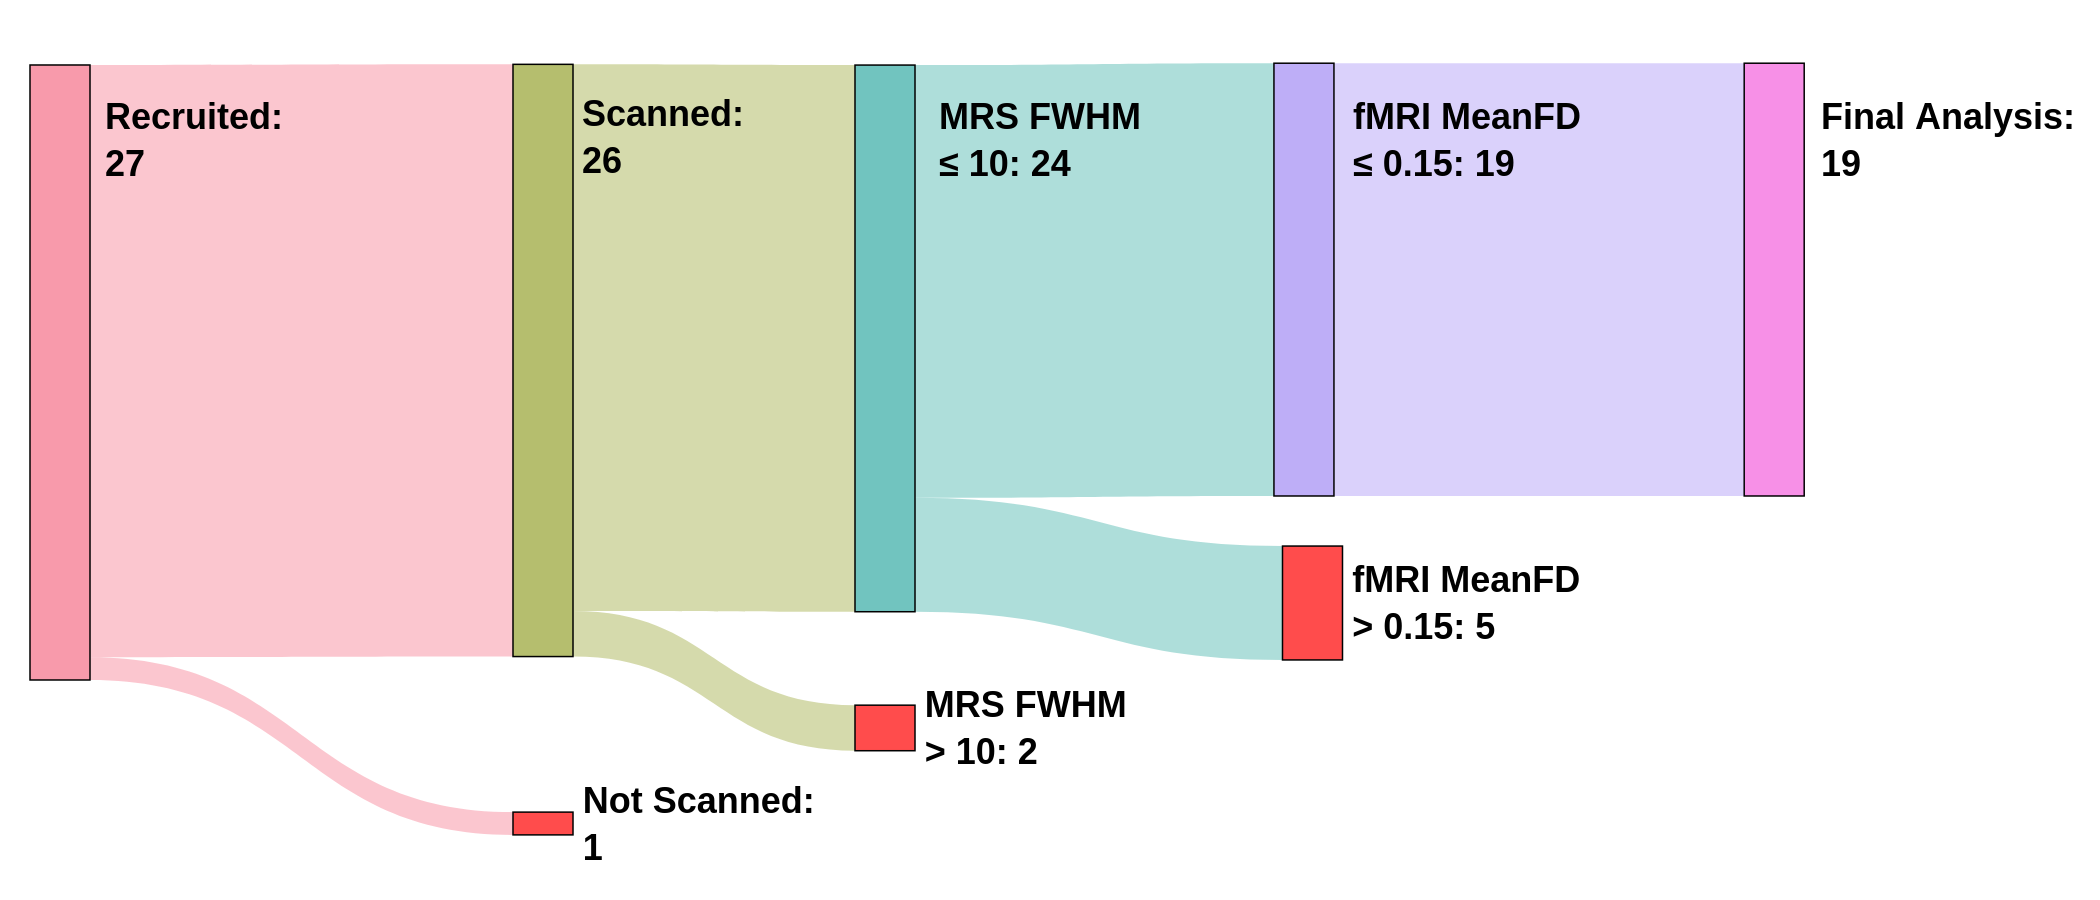
\includegraphics[keepaspectratio]{./images/ParticipantFlow.png}}

}

\caption{\label{fig-partflow}\textbf{Flowchart of participant,
recruitment, scanning and exclusion}. The number of participants at each
stage is indicated within each node. Participants were excluded based on
MRS FWHM and fMRI Mean FD thresholds, resulting in 19 participants
included in the final analysis}

\end{figure}%

The final study sample included 9 males and 10 females between ages 21.3
and 53.4, with a mean age and standard deviation of 30.1 ± 8.7 years.

\subsection{Data Quality}\label{data-quality}

\subsubsection{MRS}\label{mrs-1}

After exclusion, FWHM (mean ± sd) at rest in sLASER and MEGAPRESS were
8.52 ± 0.7 and 7.02 ± 0.7, respectively. During movie watching, FWHM in
sLASER and MEGAPRESS were 8.37 ± 0.65 and 6.98 ± 0.86.

Glx and GABA+ were tested for associations with FWHM values during rest
and movie watching. Glx during rest was found to be negatively
correlated with FWHM (r = -0.53, p = 0.02). No other correlations were
significant.

An average of all MRS voxel placements can be seen in
Figure~\ref{fig-mrsquality} A, and a sample of the \texttt{Osprey}
sLASER and MEGAPRESS spectrum fits at rest can be seen in
Figure~\ref{fig-mrsquality} B and C, respectively.

\phantomsection\label{cell-fig-mrsquality}
\begin{figure}[H]

\centering{

\pandocbounded{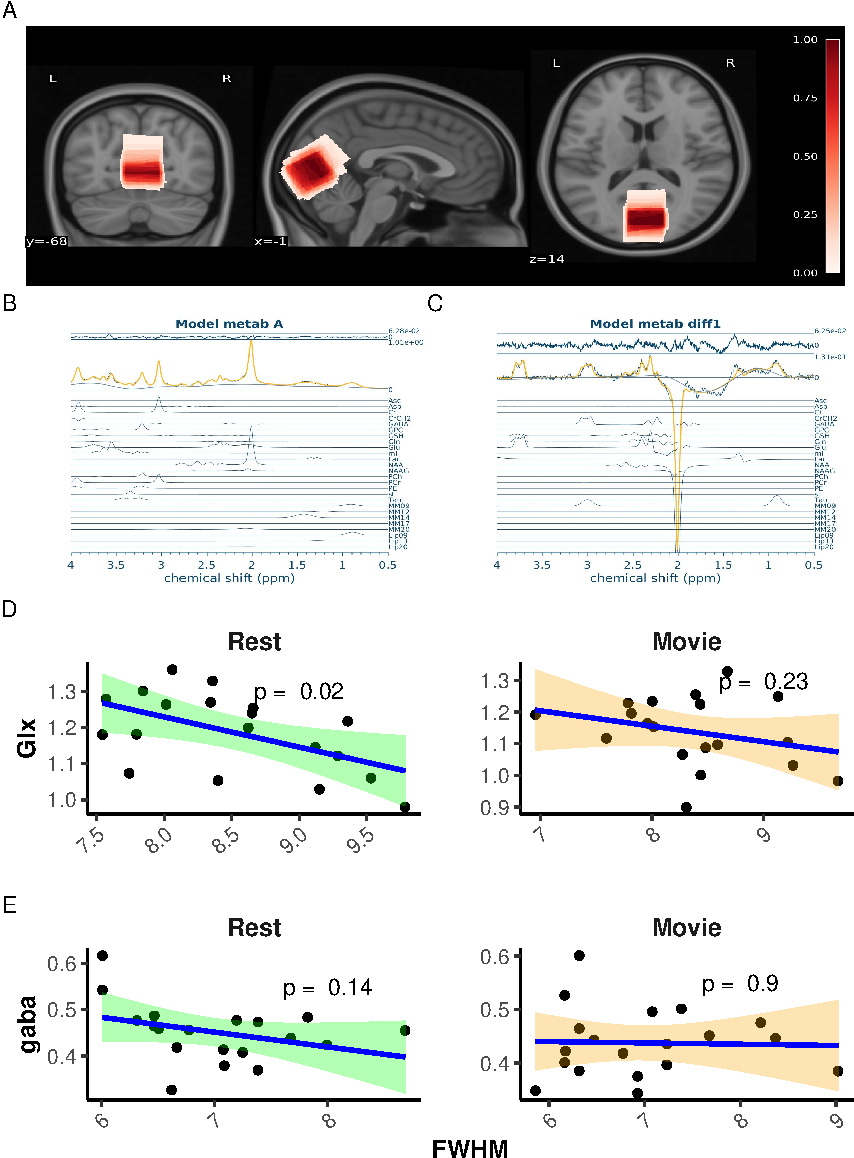
\includegraphics[keepaspectratio]{index_files/figure-pdf/fig-mrsquality-1.pdf}}

}

\caption{\label{fig-mrsquality}\textbf{MRS data quality} A) Average MRS
location. Overlay in red of the average voxel location across all
nineteen participants, from 0 (white) to 1 (dark red). Darker red
represents voxel locations shared by all participants, while white
represents voxel locations unique to participants. MRS voxels were
registered to MNI space and averaged. Underlay is T1w MNI152 at 0.5 mm
resolution. B) Sample Osprey sLASER Spectrum. Yellow spectrum indicates
overall model fit. Model fits for individual metabolites are shown in
blue below overall fit. C) Sample Osprey MEGAPRESS Spectrum. Yellow
spectrum indicates overall model fit. Model fits for individual
metabolites are shown in blue below overall fit. D) Correlation plots of
Glx / tCr vs.~FWHM for rest (green) and movie (red). E) Correlation
plots of GABA+ / tCr vs.~FWHM for rest (green) and movie (red).}

\end{figure}%

\subsubsection{fMRI and Hurst}\label{fmri-and-hurst}

A sample of the combined grey-matter and MRS voxel mask used to average
H values can be seen in Figure~\ref{fig-hurstsamp} A, along with a
sample Hurst exponent map in Figure~\ref{fig-hurstsamp} B, and sample
fits for H calculation during rest in Figure~\ref{fig-hurstsamp} C.

Mean FD was not correlated with H during rest (r = -0.33, p = 0.16 but
was moderately negatively correlated with H during movie watching (r =
-0.50, p = 0.03; see Figure~\ref{fig-hurstsamp} D).

\phantomsection\label{cell-fig-hurstsamp}
\begin{figure}[H]

\centering{

\pandocbounded{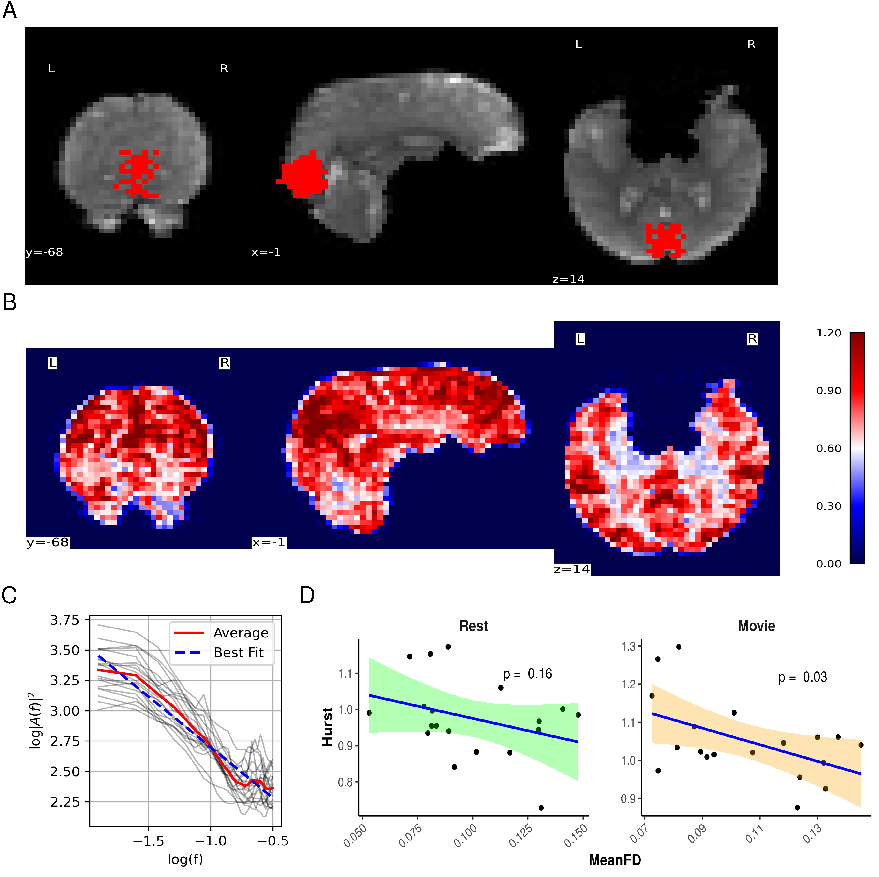
\includegraphics[keepaspectratio]{index_files/figure-pdf/fig-hurstsamp-1.pdf}}

}

\caption{\label{fig-hurstsamp}\textbf{fMRI data quality.} A) sample fMRI
grey-matter mask within the MRS voxel. Background: a sample coronal,
sagittal, and axial slice is displayed of the mean fMRI scan from the
rest acquisition. Foreground: the greymatter/MRS mask used to calculate
mean H. B) Sample H map for whole brain. Coronal, sagittal, and axial
views of are shown, colour-coded by H values. Colour-coding shows
evident tissue differentiation by H value (i.e., gray matter (red),
white matter (light red), and cerebrospinal fluid (white)). C) Sample
PSD spectrum. All participants' PSD spectrums during rest are plotted
using light grey lines. Mean PSD is plotted in solid red Mean linear
regression line is plotted in dashed blue. H for each participant was
calculated from the slope of their mean linear regression line. D)
Correlation plots of H vs.~meanFD for rest (green) and movie (orange).}

\end{figure}%

\subsection{Paired Student's T Tests}\label{paired-students-t-tests}

Mean ± sd of metabolites, E/I, and H during rest and movie are reported
in Table~\ref{tbl-results}. Neither Glx nor GAB+ were different between
movie and rest conditions (Figure~\ref{fig-results} A \& B,
respectively). E/I ratio did not change between conditions either
(Figure~\ref{fig-results} C). H was found to be greater during movie
watching than rest (Figure~\ref{fig-results} D).

\begin{longtable}[]{@{}llll@{}}
\caption{Summary of main results}\label{tbl-results}\tabularnewline
\toprule\noalign{}
& Rest & Movie & p-value \\
\midrule\noalign{}
\endfirsthead
\toprule\noalign{}
& Rest & Movie & p-value \\
\midrule\noalign{}
\endhead
\bottomrule\noalign{}
\endlastfoot
\textbf{Glx / tCr} & 1.19 ± 0.11 & 1.14 ± 0.11 & 0.09 \\
\textbf{GABA+ / tCr} & 0.45 ± 0.06 & 0.44 ± 0.06 & 0.50 \\
\textbf{E/I Ratio} & 2.68 ± 0.49 & 2.65 ± 0.45 & 0.82 \\
\textbf{H} & 0.98 ± 0.98 & 1.05 ± 1.05 & \textless{} 0.01 \\
\end{longtable}

\phantomsection\label{cell-fig-results}
\begin{figure}[H]

\centering{

\pandocbounded{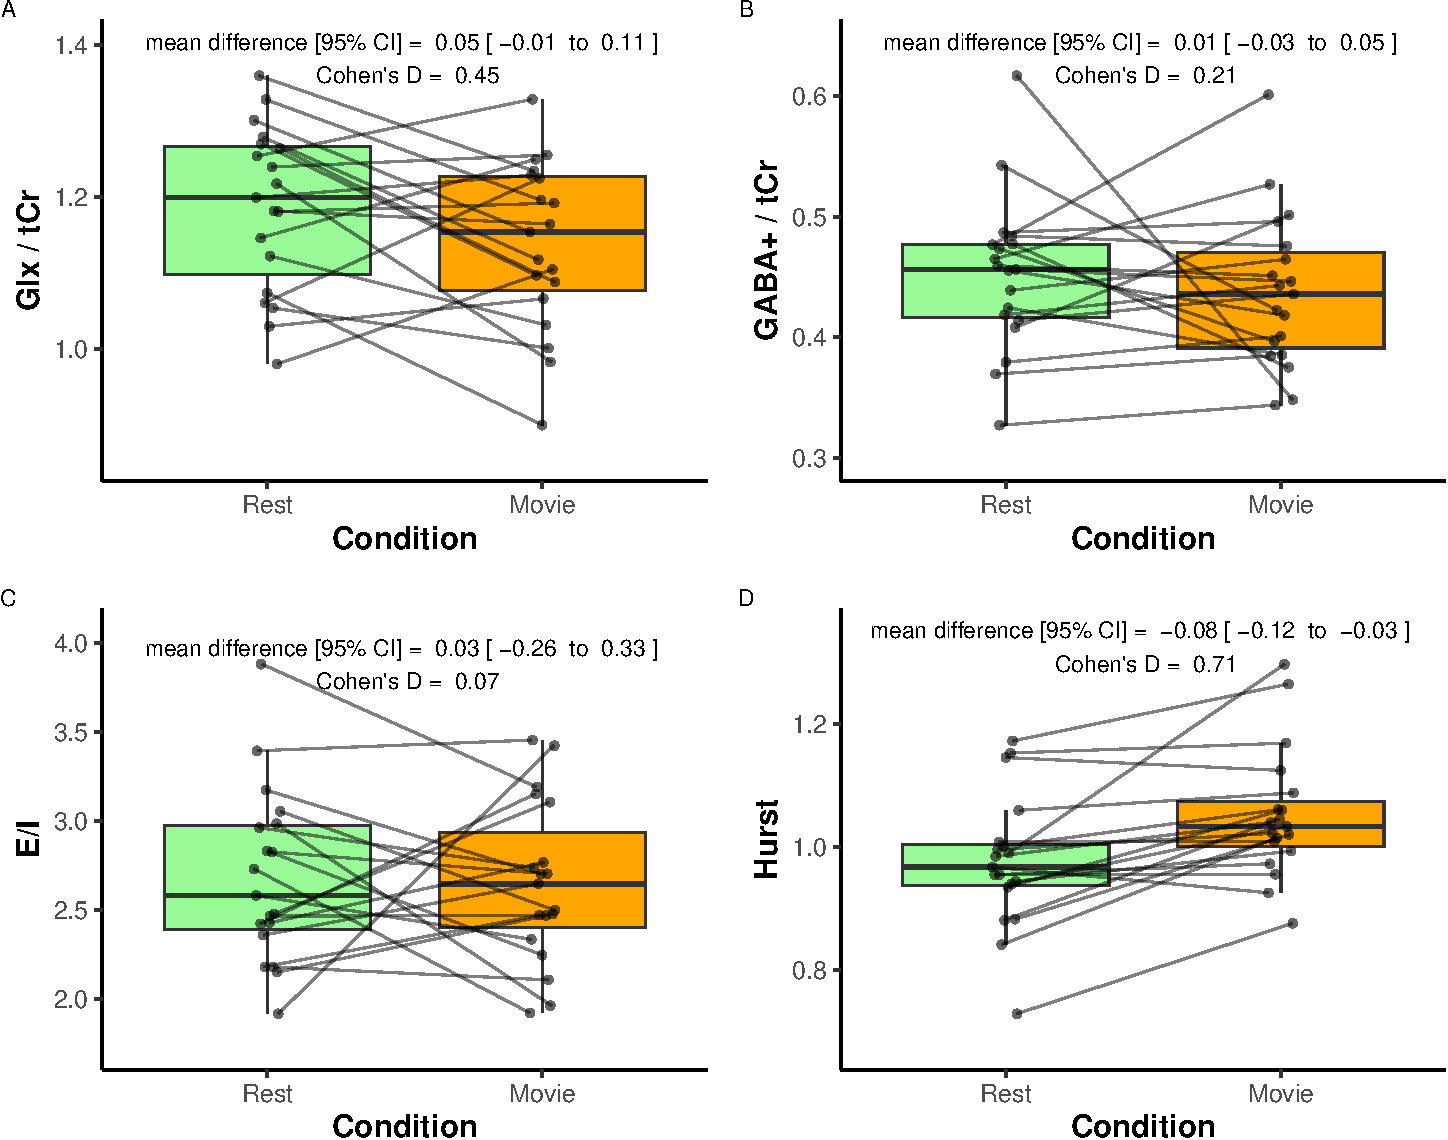
\includegraphics[keepaspectratio]{index_files/figure-pdf/fig-results-1.pdf}}

}

\caption{\label{fig-results}\textbf{Paired comparison of metabolite
values during rest (green) and movie (orange) conditions.} A) Glx / tCr;
B) GABA+ / tCr; and C) E/I. Paired dots represent the same participant
across conditions. Mean difference with 95\% confidence intervals, and
as Cohen's D are reported at the top of each plot.}

\end{figure}%

\subsection{Correlations}\label{correlations}

H was not found to correlate with Glx, GABA+, or E/I, during rest or
movie (Figure~\ref{fig-correlations}).

\phantomsection\label{cell-fig-correlations}
\begin{figure}[H]

\centering{

\pandocbounded{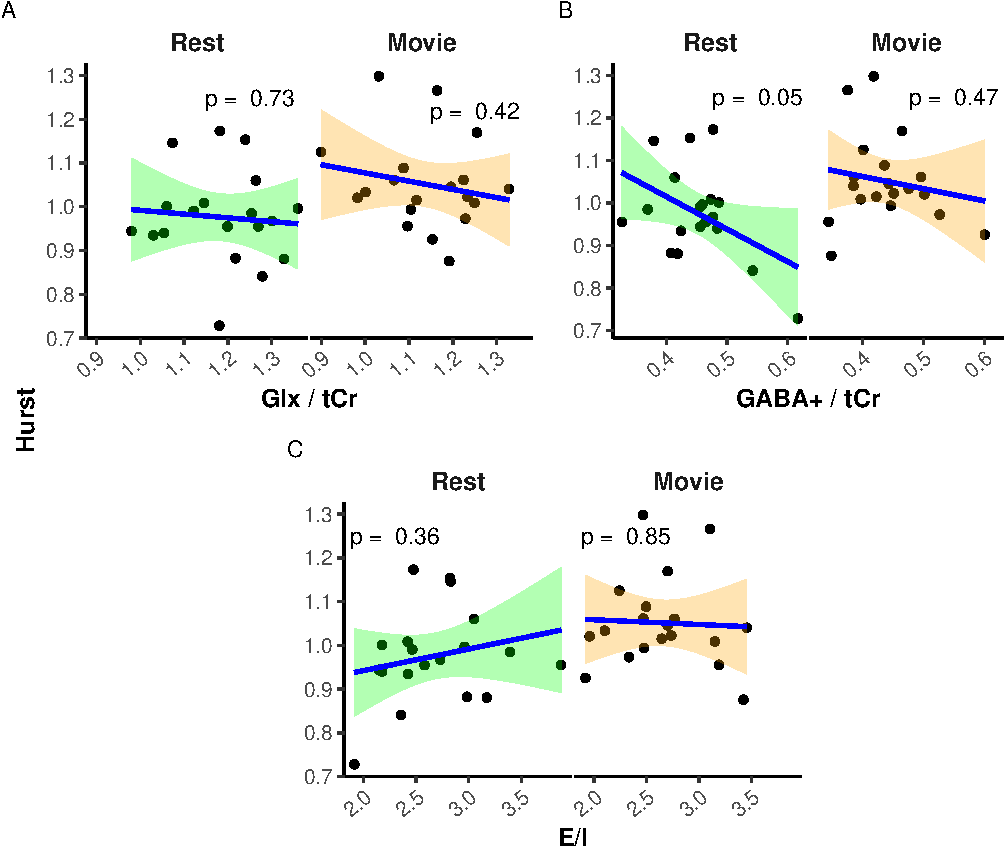
\includegraphics[keepaspectratio]{index_files/figure-pdf/fig-correlations-1.pdf}}

}

\caption{\label{fig-correlations}\textbf{Scatter plots of H
vs.~metabolites.} A) Glx / tCr; B) GABA+ / tCr; and C) E/I. Rest is in
green, while movie is in orange. p-values are reported at the top of
each plot.}

\end{figure}%

\section{Discussion}\label{discussion}

We report here the first in vivo human study of the E/I-H relationship.
An increase in H was observed during movie-watching as compared to rest,
indicating a decrease in BOLD signalling complexity in response to
visual stimuli. However, no difference in E/I was observed between
conditions, nor was H found to be related to E/I during either
movie-watching or rest. Our finding that H increases during
movie-watching compared to rest is consistent with a previous study by
our lab, which found that H increases in the visual network during
movie-watching \citep{campbellFractalBasedAnalysisFMRI2022}. However,
previous studies have observed a task-dependent H decrease using
highly-structured, active tasks requiring patient input
\citep{heScaleFreePropertiesFunctional2011, churchillSuppressionScalefreeFMRI2016, ciuciuInterplayFunctionalConnectivity2014, barnesEndogenousHumanBrain2009}.
The results of our study in combination with our lab's previous study
\citep{campbellFractalBasedAnalysisFMRI2022}, suggest that the
naturalistic, passive task of movie-watching induces a different effect
on H than more structured tasks. This is in line with literature
suggesting that distinct neural responses and BOLD signal
characteristics are observed in conventional, active visual tasks
compared to naturalistic and passive visual stimuli
\citep{campbellFractalBasedAnalysisFMRI2022, hassonReliabilityCorticalActivity2010}.

It may also be that richer scaling properties (higher H) during
movie-watching comes about to support the continuous perception of
visual stimuli during movie-watching
\citep{campbellFractalBasedAnalysisFMRI2022}. Moreover, task-induced H
changes have been observed to be dependent on task complexity and
novelty \citep{churchillSuppressionScalefreeFMRI2016}. Given this
finding, it seems reasonable to suggest that differences in task
complexity and novelty may account for discrepancies in task-induced H
changes.

We found no task-induced change in GABA+. This finding is consistent
with a large meta-analytic review which pooled the results of 49 MRS
studies \citep{pasantaFunctionalMRSStudies2023}. They too reported no
task-dependent GABA change in the visual cortex. This may due to the
technical difficulties of capturing GABA levels using MRS at 3T, owing
to its low concentration in the brain as well as signal overlap with
higher abundance metabolites \citep{pasantaFunctionalMRSStudies2023}.
However, several studies have successfully reported changes in GABA at
3T using different paradigms / regions (for example:
\citep{floyer-leaRapidModulationGABA2006, sampaio-baptistaChangesFunctionalConnectivity2015, staggRoleGABAHuman2011};
see \citet{pasantaFunctionalMRSStudies2023} for more).

We also found no change in Glx between conditions. This is somewhat
consistent with the literature -- while a meta-analysis of recent
Glu/Glx studies has reported a small task-induced increase in Glu/Glx in
the visual cortex, this finding was non-specific to visual stimuli,
including pain, learning, and motor tasks
\citep{pasantaFunctionalMRSStudies2023}. It is also true that a large
number of the studies included were conducted at 7T and thus have
greater sensitivity to detect changes in Glu/Glx than the present study.
Like GABA, glutamate is difficult to capture due to its similar chemical
structure and signal overlaps with other metabolites.

Given that no difference was observed for either glutamate or GABA
between conditions, it is unsurprising that E/I does not change either.

In terms of the central question of our research, we did not find a
relationship between H and E/I during either movie-watching or rest.
This is not entirely surprising given the large disparity of existing
findings in this regard, especially with regard to the directionality
and linearity of the proposed E/I-Hurst relationship
\citep{liangExcitationInhibitionBalance2024, poilCriticalStateDynamicsAvalanches2012, lombardiBalanceExcitationInhibition2017, baumgartenCriticalExcitationinhibitionBalance2019, bruiningMeasurementExcitationinhibitionRatio2020, trakoshisIntrinsicExcitationinhibitionImbalance, gaoInferringSynapticExcitation2017}.
The heterogeneity across these E/I-Hurst studies highlights the
challenges of studying this phenomenon as well as the complexity of any
potential relationship between these two metrics. It may be that, given
the heterogeneity of these studies in combination with our data, an
E/I-Hurst relationship --- should it exist --- is perhaps more complex
than initially thought, and may depend in part on how the data is
collected.

Another reason we may not have found a relationship between E/I and H is
that we sampled too narrow a range of profiles in terms of E/I and
Hurst. Because our study included only healthy adults, it is possible
that the participants did not show enough range in E/I and Hurst values
to see a relationship. It is also possible that while an E/I-Hurst
relationship exists, it is not observed within the visual cortex. This
theory seems plausible given that MRS studies of disrupted E/I, mostly
conducted within the context of adult autism spectrum disorder, have
found changes in E/I within other brain regions such as the anterior
cingulate cortex (ACC), frontal lobe, or temporal lobe
\citep{ajramContribution1HMagnetic2019}. Moreover, findings with
reference to changes in excitatory or inhibitory neurotransmitters
within the visual cortex tend to be difficult to capture, perhaps
indicating that E/I shows less changes in this region
\citep{pasantaFunctionalMRSStudies2023}.

\subsection{Limitations}\label{limitations}

There are two key limitations to our study which should be acknowledged.
First is the small sample size. As this was a first-attempt pilot study,
only 26 participants were initially scanned. Once individuals were
excluded for poor MRI quality, only 19 participants' data were analyzed.
With such a small sample size, it is difficult to make conclusions about
a concept as complex as the E/I-Hurst relationship as well as its
relations to criticality. The other key limitation of our study is the
low sensitivity of our MRS method --- as a result, it is hard to
conclusively state whether we found no E/I-Hurst link because it truly
does not exist or if we found no E/I-Hurst link because our methods
lacked the sensitivity to detect it. A possible solution would be to
conduct a future study using ultra-high-field 7T MRI as opposed to
conventional 3T MRI.

\section{Conclusion}\label{conclusion}

In conclusion, our findings do not support a relationship between H and
E/I in the visual cortex either during rest or during movie-watching at
3T in humans. In addition, while we found a task-related change in H, we
did not find any changes in glutamate, GABA, or E/I between movie and
rest. Comparing our findings to the broader literature, E/I balance may
be too subtle to be detected with conventional MRS methods. With regards
to the broader E/I-Hurst relationship, we similarly suggest that either
this relationship is insufficiently captured with our methods, or that
the relationship between these two variables may be more complex than
originally envisaged---perhaps they are not directly related, but rather
connected through other mediating variables in a non-linear fashion. To
our knowledge, this is the first in vivo human study to test for this
relationship. It is our hope that as the literature grows, more authors
will examine this in vivo relationship with respect to other brain
regions and using other methods, and will use the lessons learned in
this study to inform their own. Hopefully then it will be possible to
corroborate findings to probe the complex relationships that may exist
with regards to H and E/I in the human brain.


  \bibliography{EIHurst.bib}



\end{document}
